\documentclass[letterpaper,twocolumn,10pt]{article}
\usepackage{epsfig,xspace,url,lipsum}
\usepackage{authblk}
\usepackage{graphicx}
\graphicspath{ {images/} }

\newcommand\blfootnote[1]{%
  \begingroup
  \renewcommand\thefootnote{}\footnote{#1}%
  \addtocounter{footnote}{-1}%
  \endgroup
}

\title{Secure Authentication in IoT Devices}
\author{Chandrasekhar Nagarajan, Damodar Sahasrabudhe, Gurupragaash Annasamy Mani, Praveen Thiraviya Rathinam }
\affil{School of Computing, University of Utah}

\begin{document}

\maketitle
\section{Introduction}

   Internet of Things (IoTs) is an evolving technology comprising of a network of smart devices that assist in acquiring data that was not available before. The Internet of Things allows objects to be sensed and controlled remotely across existing network infrastructure,creating opportunities for more direct integration between the physical world and computer-based systems, and resulting in improved efficiency,accuracy and economic benefit. Real-time data provided by these nodes is used for comfortable, secure and intelligent living.Experts estimate that the IoT will consist of almost 50 billion objects by 2020.
   Though these devices have made life easier,it has also created new attack vectors for the hackers. IoT devices are poised to become more pervasive in our lives than mobile phones and will have access to the most sensitive personal data such as social security numbers and banking information. As the number of connected IoT devices constantly increase,security concerns are also exponentially multiplied.The following figure shows the topography of how information is collected using IOT.
   
   Each IoT device is identified in the network using an unique IP address or a RFID tag[add reference]. The gateway is the entity via which the individual IoT nodes communicate with the external world. Many IoT devices allow access and control from multiple sources in the network via the Cloud[add reference if available]. Cisco estimates that there will be atleast 50 billion devices connected to the Internet by 2020[add reference].
   
   
   Our initial motivation for this work was the "Hacking" of the Amazon Dash button[add reference]. A person had changed the intended purpose of the Dash button to do something else which was not intended for the device.He had explained in his blog how it was easier to hack into the device and change the code.We felt that this can be used by an attacker to do some malicious activities.On further investigation regarding the IoT devices,we found that commercial companies are focusing more towards deploying newer IoT devices than strengthening the security measures in existing devices.As per a survey done by HP regarding the current deployment of IoT devices approximately 70\% of them operate under insecure networks[add reference]. The weak authentication features, communication over unsafe mediums and poor password schemes lead to vulnerabilities that have the urgency to be resolved. The fundamental reason given for such weak mesures is that IOT devices have lower compute power,memory and lesser capabilities that computers,routers and servers.
   
   In our project,we wanted to analyze how a server can differentiate between data from an authentic IoT device and fake data from another malicious device because this would ensure that
the server does not record any fake data and generate false alerts. We are focusing on the IoT devices which would generally send periodic updates of some environment statistics like presssure,
temperature etc because we felt that these are the more frequently used devices in home management systems.We are also not encrypting the data values being transmitted in the network and focusing only 
on the different schemes that can be used for signing the message being sent to the server. We wanted to evaluate the different authentication methods from an IoT perspective because these devices
generally have lower configuration so some schemes might not be possible in them.The main goal of our project was the following :

\begin{itemize} 

\item  Focus on various authentication schemes like RSA, Zero Knowledge signature(ZKS) that can be used in IoT devices.

\item  Implement a RSA signature scheme for authenticating data transmitted by IoT devices.

\item  Implement a ZKS signature scheme for authenticating data.

\item Do a comparitive study of the ZKS and RSA techniques in terms of 
\begin{itemize}  
 \item Running time 
 \item Power Consumption
 \item Memory Usage
\end{itemize}   
\end{itemize}   

From this project,we were trying to establish the fact that the ZKS signature scheme is better than the RSA signing method in terms of processing time, power and memory usage and so would be ideal for use
in an IoT device.
 
\begin{figure}[htbp]
	\begin{center}
        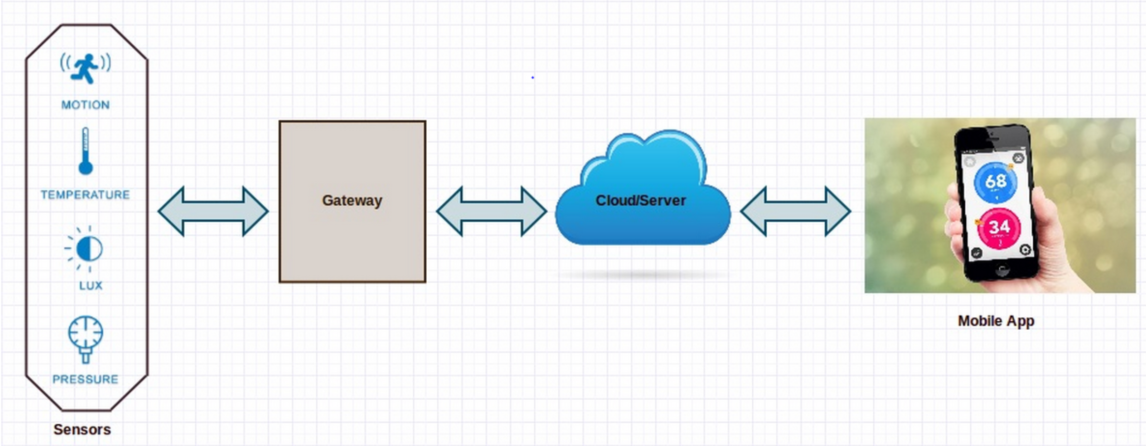
\includegraphics[width=80mm]{intro.png}
		\caption{introduction}
		\label{Introduction}
	\end{center}
\end{figure}
\section{Related Work}
Several studies have been conducted on what are the problems present in the IOT devices.The Open Web Application Security Project(OWASP) IOT project was formed to identify the problems seen in IOT devices.[add reference].The project identified several attack surface areas,vulnerabilities like insecure web interface, insufficient authentication methods,insecure mobile network,insecure security configurations and lack of transport security protocols. The goal of this project was to provide a set of guidelines to the developers,testers,manufacturers and the consumers to ensure that the IOT devices are safely and ethically used.
  
  \section{Adversary Model}

  In our threat model,the adversary would be able to listen to all the communications happening in the network. The adversary would have access to the wireless medium between the IOT and Server which is collecting the data from the IOT.Since we focused on the sensor devices,the possible values that a device might transmit would be between a certain range so it would be possible for an adversary to find out what data is going through the wireless channel.Also since we are not encrypting the data and only focusing on signing the messages being transmitted, seeing the values should be easy for the adversary.If the adversary is able to find the private keys in case of RSA or the secret maintained in case of ZKS, we would not be able to securely transmit the data.  
  \section{Methodology}
	As many of the devices used in IoTs have limited resources, implementing compute and memory intensive algorithms such as RSA is not practical and need some lightweight solution to carry out data authentication. Here we aim to implement ZKS, RSA and variation of ZKS - we call it Optimized ZKS or OZKS and compare there performance in terms of CPU run time, memory allocation and power consumption.
\paragraph We used Raspbery Pi as a device, used a dummy data, say temperature, to be sent from device to "hub" located on laptop. To ensure authentication of message we signed message using RSA / ZKS / OZKS and then sent message to server. Server can verify signature and authenticate whether data is sent over by authentic device or not.
\paragraph{OZKS} During experimentation we found that random number generation is taking significant around 25 to 30 percent of compute time. So we came up with Optimized ZKS. In OZKS instead of calculating 128 random numbers, we store pre-calculated 128 numbers in an array. Every time a single random number is generated and then XORed with each of number stored in array to generate pseudo random number. We can see in CPU and memory graphs that OZKS saves around 25 to 30 percent of CPU run time without much increase in memory utilization and power consumption.

\section{Implementations}




\section{Pictures}

\begin{figure}[htbp]
	\begin{center}
        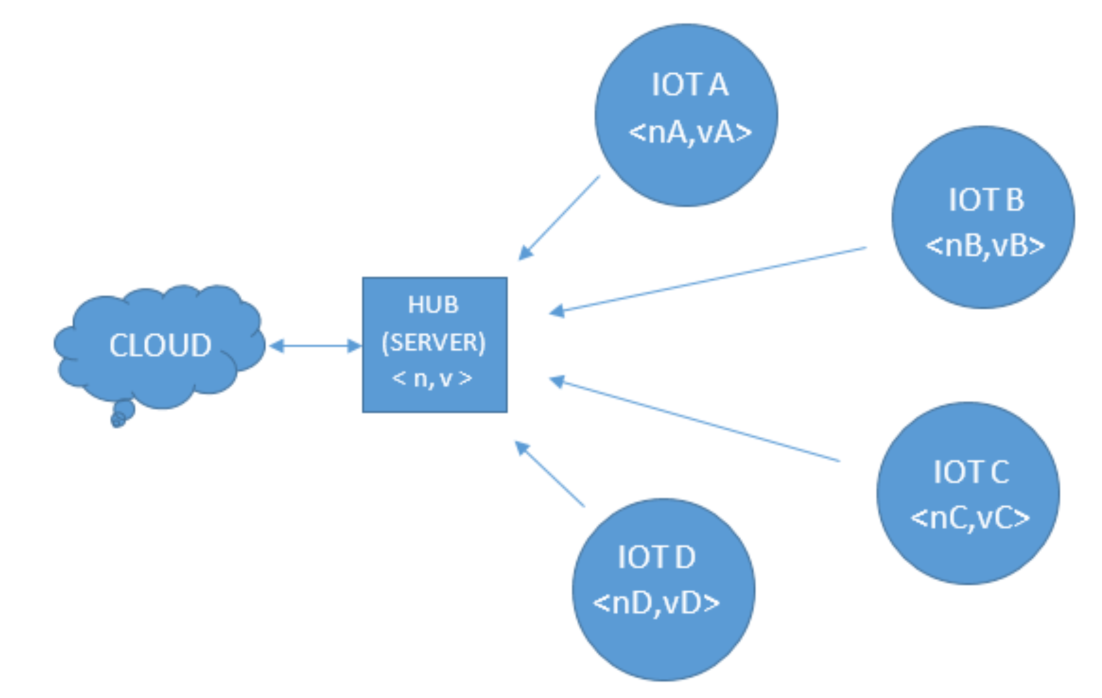
\includegraphics[width=80mm]{Networkarchitecture.png}
		\caption{Architecture}
		\label{System Architecture}
	\end{center}
\end{figure}

\begin{figure}[htbp]
	\begin{center}
        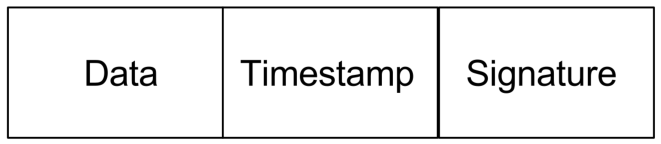
\includegraphics[width=80mm]{Rsa_packet.png}
		\caption{RSA packet format}
		\label{rsa_packet}
	\end{center}
\end{figure}


\begin{figure}[htbp]
	\begin{center}
        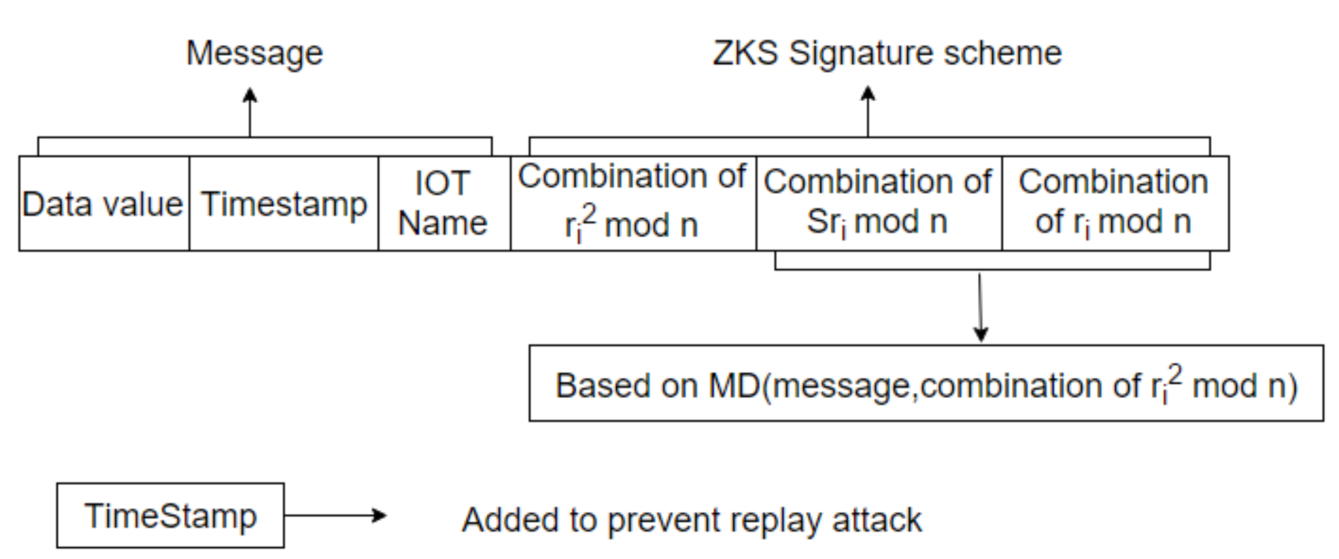
\includegraphics[width=80mm]{zks_packet.png}
		\caption{ZKS packet format}
		\label{zks_packet}
	\end{center}
\end{figure}
\section{Conclusion}



{
  \footnotesize 
  \small 
  \bibliographystyle{acm}
  \bibliography{biblio,project}
}
\end{document}



